\documentclass[12pt,a4paper,spanish]{book} %%%Esto indica el tipo de documento.Va a ser un libro (book), el tama�o es a4, la lengua castellano (spanish)%%%
\usepackage[spanish]{babel} %%%Incluimos el paquete Babel que sirve para separar correctamente las palabras de multitud de idiomas%%%
\usepackage[latin1]{inputenc}%%%Este paquete permite poner acentos directamente%%%
\usepackage[T1]{fontenc}
\usepackage{amsmath}%%%Macros AMS%%%
\usepackage{amsthm}%%%Macros AMS para teoremas%%%
\usepackage{amsfonts}%%%Permite usar fuentes AMS%%%
\usepackage{amssymb}%%%Para usar simbolos AMS%%%
\usepackage{shadow}
\usepackage{indentfirst}%%%Espaciado deprimera l�nea de cada p�rrafo%%%
\usepackage{fancyhdr}
\linespread{1.5}
\usepackage{graphicx}
\usepackage{appendix} %%%Permite un manejo sencille de los ap�ndices. Permite tambi�n introducir subapendices.
\usepackage[colorlinks=true]{hyperref}%De esta forma el PDF sale muy chulo
\usepackage{graphics}
\usepackage{anysize} % Soporte para el comando \marginsize
\usepackage{theorem}
\usepackage{float}
\marginsize{3cm}{2cm}{2.5cm}{2.5cm}%Permite manejar los m�rgenes de forma sencilla
\usepackage[Lenny]{fncychap}
\usepackage{url}
\usepackage{listings} %Permite a�adir c�digo
\lstset{language=bash,
           basicstyle=\ttfamily,
           keywordstyle=\color{blue}\ttfamily,
           stringstyle=\color{red}\ttfamily,
           commentstyle=\color{green}\ttfamily,
           breaklines=true
          }
%\usepackage{eurofont}%Permite usar el s�mbolo de euro
 \pagestyle{fancy}
%\addtolength{\footskip}{+3cm}
\usepackage{fancyhdr}                                   %Para un encabezado especial m�s visual
\usepackage{extramarks}

\author{C�sar Mart�n Crist�bal}
\title{\textbf{Persistencia e integridad de datos en memorias Flash}}
%-----------------------------------------------------------------------------------------------
%-----------------------------------------------------------------------------------------------
\begin{document}%%%Aqu� empieza el documento%%%

%%%Portada%%
%------- T�TULO     ----------
%=============================
\begin{titlepage}
\begin{center}
{\large\textbf{Universidad de Valladolid}}
 \vspace{0.8cm}
{\large\textbf {Escuela T�cnica Superior de Ingeniero de Telecomunicaci�n}}\\
 \vspace{0.8cm}
{\large\textbf{Ingenier�a T�cnica  De Telecomunicaci�n}}\\
{\large\textbf {Sistemas De Telecomunicaci�n}}
\end{center}


\begin{figure}[here]
\centering
%
\includegraphics[scale=0.3]{figuras/escudo.eps}

\includegraphics[scale=0.3]{fig/portada_logoetsit.eps}

\end{figure}


\begin{center}
{\large\textbf {PROYECTO FINAL DE CARRERA}}\\ \vspace{1.5cm}

{\Large \bf Persistencia e integridad de datos en memorias Flash}\\ \vspace{0.2cm}
\end{center}


\begin{table}[h]
    \begin{flushright}
        \begin{tabular}{l @{\quad} l}
            \textbf{AUTOR:} & \textbf{C�sar Mart�n Crist�bal}\\
            \textbf{TUTOR:} & \textbf{Juan Carlos Escart�n}\\
        \end{tabular}
        \end{flushright}
\end{table}
\begin{flushright}
{\large \textbf{12 de septiembre de 2014}}
\end{flushright}

\end{titlepage}
%Portada Gr�fica

\DeclareGraphicsExtensions{.jpg,.pdf,.mps,.png,.gif,.fig,.bmp,.PNG}
%Declaraci�n de extensiones de figuras para el paquete graphicx

%\renewcommand\tablename{Tabla}%De esta forma sale nombre de Tabla en vez de Cuadro
%\renewcommand\listfigurename{Lista de Figuras}
%\renewcommand\listtablename{Lista de Tablas}

\thispagestyle{empty} \cleardoublepage
%Se deja sin numeraci�n las p�ginas siguiente

%==============================================================
% Acta
%===============================================================
\thispagestyle{plain}
%\begin{large}

  \noindent  \begin{tabular}{p{2cm}p{11cm}}
        \textsc{T�tulo:} & \emph{QUIERO HACER MI PFC EN \LaTeX, PERO �POR D�NDE EMPIEZO?}. \\
        & \\
        \textsc{Autor:} & \emph{�SCAR BARQUERO P�REZ} \\
        & \\
        \textsc{Tutor:} & \emph{ALBERT EINSTEIN}\\
        & \\
        \textsc{Cotutora:} & \emph{MADAME CURIE}
    \end{tabular}

\end{large}

\vspace{1cm}

La defensa del presente Proyecto Fin de Carrera se realiz� el d�a
19 de Enero de 2005; siendo calificada por el siguiente tribunal:

\vspace{0.8cm}

\noindent \begin{tabular}{p{3cm}p{10cm}}

    & \\
    \textsc{Presidente:} & \emph{Profesor Bacterio} \\
    & \\
    & \\
    \textsc{Secretario} & \emph{Mortadelo} \\
    & \\
    & \\
    \textsc{Vocal} & \emph{Filem�n} \\
\end{tabular}

\vspace{0.8cm}

Habiendo obtenido la siguiente calificaci�n:

\vspace{0.8cm}

\noindent \begin{tabular}{p{3cm}p{10cm}}

    & \\
    \textsc{Calificaci�n:} & \emph{} \\
    & \\
    \end{tabular}

\vspace{1.2cm}

\begin{bfseries}
    \begin{center}
        Presidente \hspace{3cm} Secretario \hspace{3cm} Vocal
    \end{center}
\end{bfseries}

%\newpage
\thispagestyle{empty}\cleardoublepage

%==============================================================
%Agradecimientos
%==============================================================
\thispagestyle{plain}
%\begin{center}
   \Large{\textbf{Agradecimientos}}
\end{center}

Agradecimientos
\newpage
\thispagestyle{empty}\cleardoublepage

%==============================================================
%Resumen
%==============================================================

\chapter*{Resumen}

En este proyecto hemos profundizado sobre el funcionamiento de las memorias Flash, sobre todo en lo que se refiere al funcionamiento interno, a bajo nivel. Nos hemos centrado en determinar en qu� posiciones de memoria guarda la tabla de nombres, c�mo gestiona los archivos, cu�l es el tama�o que tiene un sector y cu�ntos ciclos de vida �til tiene un sector. Para esta investigaci�n hemos desarrollado una serie de scripts en Bash Shell de Linux que nos han permitido obtener y evaluar los resultados de manera m�s sencilla. Los resultados a los que hemos llegado despu�s de la investigaci�n son que este tipo de tecnolog�a se usa en todo tipo de dispositivos, y tiene mucha progresi�n de futuro. Tras los experimentos, hemos llegado a las siguientes conclusiones: el tama�o de bloque de memoria que impone el sistema de ficheros se mantiene a nivel f�sico, el montado y desmontado del dispositivo no generan cambios en �l y son m�s fr�giles los componentes que acompa�an a la memoria que la propia memoria.

memoria flash, persistencia de datos, l�mite de escritura, tabla de ficheros.



In this project we have deepened over the operation of Flash memories,
especially as it relates to the internal operations at low level. We focused
to determine which memory locations stores table names, how it manages
files, what is the size it is a sector and how many life cycles have a
sector. For this research we have developed a series of scripts in Bash Shell
Linux that have allowed us to obtain and evaluate the results more easily.
The results which have come after the research are that this type
technology is used in all kinds of devices, and has lots of future progression.
After the experiments, we have reached the following conclusions: the block size
memory imposed by the file system remains physically, mounted and
removed from the device does not generate changes, and are more fragile components
accompanying the report that the memory itself.

\newpage\thispagestyle{empty}
\cleardoublepage

%===============================================================
%�ndices
%===============================================================
\pagestyle{plain}
%\tableofcontents
%\listoffigures
%\listoftables

%===============================================================
%Para el encabezado que se va a utilizar en todo el proyecto
%===============================================================
\pagestyle{fancy}

\renewcommand{\sectionmark}[1]{\markright{\thesection\ #1}}
\fancyhf{} \fancyhead[LE,RO]{\bfseries\thepage}
\fancyhead[LO]{\bfseries\rightmark}
\fancyhead[RE]{\bfseries\leftmark}
\setlength{\parskip}{4mm}
%=============================================================

%=============================================================
%Cap�tulos
%=============================================================

\chapter{Introducci�n}

En este cap�tulo se har� una breve exposici�n sobre el proyecto final de carrera.

un poco de bla bla bla bla bla

Empezaremos con una introducci�n a la tegnolog�a Flash.

\section{�Qu� son las memorias Flash?}

La memoria flash es una evoluci�n de la memoria EEPROM, permite la lectura y escritura de m�ltiples posiciones de memoria en la misma operaci�n. Gracias a ello, la tecnolog�a flash, permite velocidades de funcionamiento muy superiores a la tecnolog�a EEPROM, que s�lo permit�a actuar sobre una �nica celda de memoria en cada operaci�n de programaci�n.

Utiliza una tecnolog�a de almacenamiento que mediante impulsos el�ctricos es capaz de leer, escribir o borrar informaci�n. Estas memorias est�n basadas en transistores de puerta flotante colocados formando celdas. El elemento b�sico de funcionamiento de las memorias son los transistores MOS de puerta-flotante \cite{IntroductionFlash}.

Fujio Masuoka en 1984 invent� este tipo de memoria como evoluci�n de las EEPROM existentes por aquel entonces, mientras trabajaba en Toshiba. Intel intent� atribuirse la creaci�n de esta sin �xito, aunque si comercializ� la primera memoria flash de uso com�n en 1988 [2].

Se dividen en dos clases seg�n el tipo de puertas usado en su fabricaci�n:
\begin{itemize}
  \item NAND: dise�adas con unas celdas muy peque�as, que permiten tener un precio muy peque�o por bit de almacenamiento.
  \item NOR: t�picamente se han usado para almacenar el software que luego es ejecutado en los dispositivos port�tiles.
\end{itemize}
En la actualidad la diferencia entre los dos tipos es cada vez menor \cite{FlashMemoryWikipedia}.


Que mierda pasa con el lineado !!!

asdfa

adfa
ads
adf


\begin{figure}
	\centering
		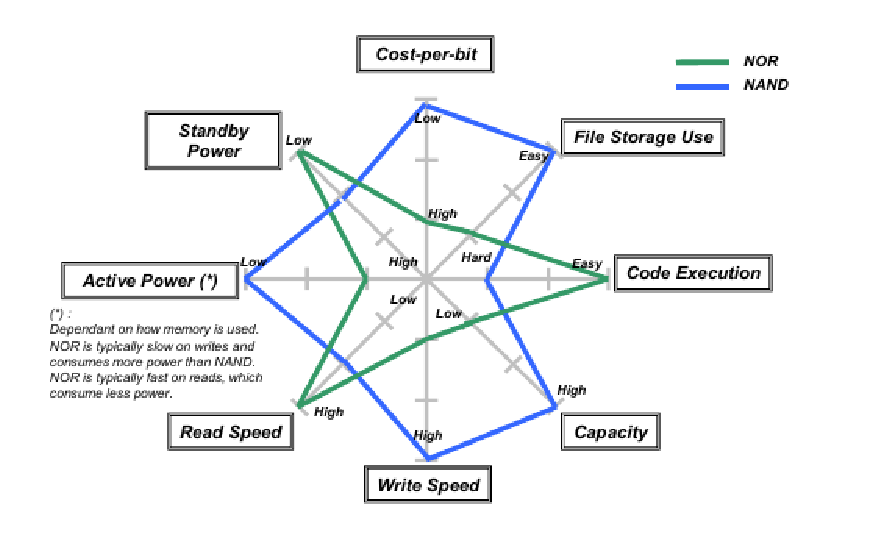
\includegraphics[width=0.60\textwidth,natwidth=610,natheight=642]{fig/comparacionNORNAN}
	\caption{\emph{Diferencia entre Flash NOR y NAND}}
\end{figure}


\chapter{Antecedentes}
\section{Estado del arte}

\subsection{Descripci�n de equipos}
Para poder realizar los experimentos hemos contado con dos equipos en el laboratorio. Son dos equipos con procesador AMD Phenom (tm) X6 1055T y 7'6 GiB de RAM. En ellos hemos instalado Debian 6.0.6, que viene con el kernel 2.6.32-5-amd64.

Ambos dos forman parte de una red interna de \url{gf.tel.uva.es}, teniendo cada uno de ellos los siguientes hostnames:
\setlength{\parskip}{0mm}
\begin{itemize}
\item Leonardo, con la IP: 192.168.0.50.
\item Donatello, con la IP: 192.168.0.51.
\end{itemize}
\setlength{\parskip}{4mm}

Como esta red no est� accesible desde el exterior de la escuela, para poder trabajar desde casa y tener monitorizado el trabajo, hemos recurrido a los tuneles ssh y al commando screen de Linux, que detallamo en la siguiente secci�n \ref{subsec:ComoTrabajarDesdeFueraETSiT}.

\subsection{Caracter�sticas de la memoria}

La diferencia entre lo que se ve desde el software y lo que fisicamente est�, es algo muy importante en este Proyecto. Como ya hemos comentado, todas las memorias disponen de un controlador, y este puede recolocar los datos de manera interna, y completamente trasparente desde el exterior.

Este tipo de memorias est�n formateadas con FAT32. FAT es un sistema de archivos desarrollado para MS-DOS. FAT32 es su �ltima evoluci�n, utiliza direcciones de cluster de 32 KiB (aunque s�lo 28 de esos KiB se utilizan realmente) y el tama�o m�ximo de un archivo en FAT32 es 4Gigabyte.

Tama�o de cluster que impone fat32 \cite{fat32_1} \cite{fat32_2}

\section{Utilidades}

\subsection{Comandos y herramientas utilizadas}
\subsubsection{Comando Linux}
En Linux existen mulitud de comandos que nos han facilitado el trabajo a la hora de realizar este Proyecto. Uno de los m�s importantes ha sido \verb|dd|.
\begin{itemize}
\item \verb|dd|: \textit{Copia un fichero, convirtiendo y formateando seg�n los operandos}.
En principio este comando se usa para crear copias de un disco, en nuestro caso creamos archivos \verb|.iso| de las memorias USB. Pero en unas pruebas nos dimos cuenta de que ten�a mayor rendimiento que el comando \verb|cp|, que es el originario de Linux para copiar ficheros, y desde ese momento lo hemos usado tambi�n para la copia ``normal''. Por defecto sus bloques de copiado son de 1024bytes y sus par�metros son los siguientes:
\begin{verbatim}
$ dd if=ruta_o_fichero_entrada of=fichero_salida
\end{verbatim}
\item \verb|df|: \textit{Uso del espacio del sistema de ficheros}.
Este comando te da informaci�n sobre el espacio de los dispositivos montados en el sistema. A parte de ver el espacio disponible en las memorias, principalmente se ha utilizado para ver la capacidad de las memorias y comprobar si su capacidad se ha visto recudida, ver /ref{experiementoFlash}. Nota importante:
\begin{verbatim}
$ df --block-size=kB \\ Muestra un tama�o de bloque de 1000bytes
$ df --block-size=k \\ Muestra un tama�o de bloque de 1024bytes
\end{verbatim}
\item \verb|hexdump|: \textit{Muestra el contenido de un fichero en ascii, decimal, hexadecimal, u octal}.
Gracias a la orden:
\begin{verbatim}
$ hexdump -c .iso > .txt
\end{verbatim}
Podemos crear un archivo de texto que luego comprar con \verb|meld|, de esta manera podemos comparar im�genes \verb|iso| de forma muy f�cil y ver sus diferencias.
\item \verb|iotop|: \textit{Muestra el proceso de las peticiones de lectura o escritura que implican a distintos dispositivos del sistema}.
Gracias a este comando podemos monitorizar si una lectura o escrita a la memoria sigue en curso o murio su proceso.
\item \verb=ls -l | wc -l=: Esta orden muestra la cantidad de elementos en un directorio, ha sido de mucha utilidad sobre todo en el experimento de /ref{tabladenombres}.
\item \verb|od -x .txt|: \textit{Muestra un fichero en octal y otros formatos}.
Hemos utilizado ficheros en hexadecimal, como ficheros base de lectura y escritura en este proyecto, este comando ha ayudado a visualizar esos ficheros hexadecimales.
\end{itemize}
\cite{manLinux}
\cite{Programaci�ndeShellScripts}

\subsubsection{Bash y Shell script}
\textbf{Bash} es un it�rprete de �rdenes, est� basado en la shell de Unix y es compatible con POSIX. Su nombre viene del acr�nimo ``\textit{Bourne-Again SHell}'', un juego de palabras de Stephen Bourne, el autor del antecesor de la Shell actual de Unix \cite{gnubash}. Bash dispone de una gran cantidad de comandos que te permiten hacer casi cualquier cosa \cite{indexbashcommand}.

Una \textbf{Shell} es un marco que ejecuta comandos. La Shell puede aceptar de entrada �rdenes por teclado o leer instrucciones de un fichero \cite{gnubash}.

Un script de Shell es una secuencia de comandos que se ejecutan uno detr�s de otro, ya que es un tipo de lenguaje interpretado. Un fichero de texto con extensi�n \verb|.sh| al que se le da permisos de ejecuci�n ``\verb|chmod u+x script.sh|'' ya es puede ser ejecutado en Linux.

Gracias a estos Shell script hemos podido automatizar procesos que podr�an llevar muchos d�as y filtar los resultados para una mejor comprensi�n de los mismos.

Bash tiene algunas peculiaridades a la hora de tratar con variables que puede llamar la anteci�n acostumbrado a otros lenguajes de programaci�n:

\begin{itemize}

\item La asignaci�n de variables se realiza sin ``declaraci�n'': \verb|varible=valor|.
\item Para modificar esas variables se usan dobles parentesis: \verb|((variable=variable+10))|.
\item Para usar las variables deben estar precedidas de \verb|$|: \verb|echo ``Hola'' $variable|.

\end{itemize}

\subsubsection{Control de versiones y Git}
Git es una herramienta para el control de versiones. Tiene muchas virtudes, pero la m�s importante en este contexto es poder tener un hist�rico de cada cambio ``comiteado'', lo que nos permite tener una copia de seguridad casi perfecta tanto del c�digo como de la redacci�n de Proyecto. En cualquier momento podemos volver a un punto anterior o ver que se cambiado de un fichero en concreto \cite{git-scm}. Todo el Proyecto se ha ido guardando en \url{github.com}, que permite crear repositorios git de manera gratuita siempre que estos sean de libre acceso, esta direcci�n del repositorio: \url{https://github.com/jilgue/flashcrash}.

\subsection{�Com� trabajar desde fuera de la ETSiT?}
\label{subsec:ComoTrabajarDesdeFueraETSiT}
Se puede tardar d�as en conseguir resultados, para monitorizar el proceso es necesario conectarse a los equipos y poder recuperar la shell donde tenemos lanzado el script. Para ellos nos hemos ayudado del protocolo SSH y el comando screen.

\subsubsection{SSH}
SSH es un protocolo de shell remota segura. Gracias a ello podemos conectarnos al terminal de un ordenador y ejecutar ordenes en �l. 

SSH usa una autenticaci�n con cable publico/privada. Si queremos conectarnos por SSH sin tener que escribir la contrase�a cada vez, tenemos que generar una pareja de claves y a�adir la publica a nuestro servidor:
\begin{verbatim}
$ ssh-keygen -t rsa -b 2048
\end{verbatim}

Esto nos genera un \verb|.pub| dentro de la carpeta \verb|.ssh| y tenemos que copiar su contenido en el archivo \verb|.ssh/authorized_keys| del servidor. Con esto la pr�xima vez que nos conectemos no tendremos que escribir la contrase�a \cite{Criptograf�aasim�trica}.

\subsubsection{Tunelando con ssh}
En la escuela tenemos una arquitectura parecida a esta \ref{fig:Esquemadered}:

\begin{figure}
	\centering
		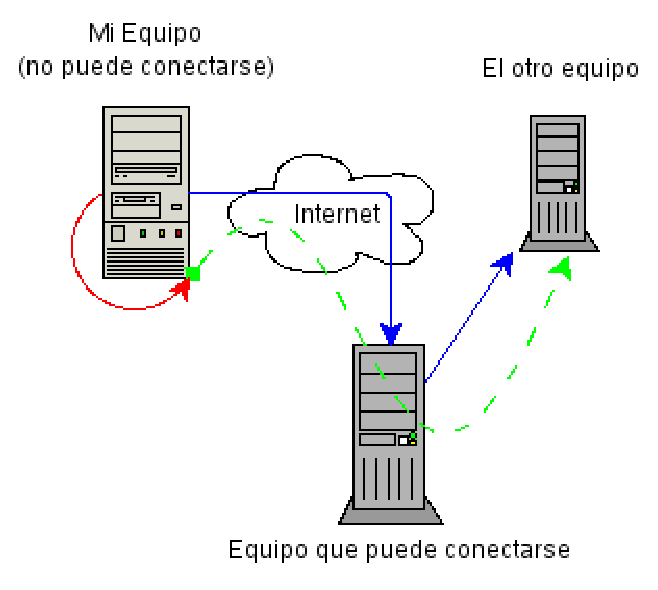
\includegraphics[width=0.60\textwidth,natwidth=299,natheight=266]{fig/tunel-ssh2}
	\caption{\emph{Esquema de red}}
        \label{fig:Esquemadered}
\end{figure}

Desde ``Mi equipo'' no puedo conectarme al ``Otro equipo''. Para solvertar este problema creamos un tunel:
\begin{verbatim}
$ ssh -L 2222:donatello:22 -L 2221:leonardo:22 usuario@gf.tel.uva.es
\end{verbatim}

Con esta linea hemos abierto un t�nel desde nuestro puerto 2222 y 2221 al 22 de donatello y leonardo respectivamente a trav�s de \url{gf.tel.uva.es}. Ahora para conectarnos a nuestro t�nel escribimos en nuestro terminal:
\begin{verbatim}
$ ssh usuario@localhost -p2221 -X
$ ssh usuario@localhost -p2222 -X
\end{verbatim}

\subsubsection{Screen}
Screen es una herramienta que nos permite recuperar una sesi�n shell. Podemos dejar corriendo un script cerrar la conexi�n, irnos a casa, abrir una conexi�n nueva y recuperar la misma terminal que ten�amos antes.

Uso b�sico de \verb|screen|:
\begin{verbatim}
$ screen // abre una sesi�n
Ctrl + a + d // deja la sesi�n en background.
$ screen -r // recupera la sesi�n
\end{verbatim}
\cite{Usodet�nelessshyscreen}
\cite{Usob�sicodescreenenLinux}

\chapter{Desarrollo}

\section{Experimentos}


\section{C�digo}
\verb|archivos_marcados_b3.sh|
\begin{lstlisting}
#
# Crea ficheros de todos los tama�os posibles hasta llegar a 'valor_final'
#
valor_final=3907388
((tamfinal=valor_final*1024))

aux=2
cont=0
while [ $aux -le  $tamfinal ]; do

	((aux=aux+aux))
	((cont++))
done

echo "auxiliar" $aux
echo "contado" $cont
rm datos/*
echo -e -n "\x00" > datos/datos0.txt

((aux=cont))

echo "vamos a contar desde 1 a " $aux

for (( a=1 ; a<=aux ; a++ ))
do
	((b=a-1))
	cat datos/datos$b.txt > datos/datos$a.txt
	cat datos/datos$b.txt >> datos/datos$a.txt
	echo $b
	echo $a
done
\end{lstlisting}


\verb|flash_b2.sh|
\begin{lstlisting}
#
# 
#
dispo="4E06-0AB9"
sdd="sdb"
rm stam.txt	
for (( b=0 ; b<999999999999999999999 ;b++))
do
	let vueltas=$b

for (( a=1 ; a<3 ; a++ ))
do
	echo "numero serie ${b}_${a}"
	echo -e -n "numero serie ${b}_${a}" > datos/${b}_${a}datos.txt
	for (( c=1 ; c<200 ; c++ ))
	do
		echo -e -n "numero serie ${b}_${a}" >> 
datos/${b}_${a}datos.txt
	done
	#cat datos/datos.txt >> datos/${b}_${a}datos.txt
	#echo -e -n "numero serie ${b}_${a}" >> datos/${b}_${a}datos.txt
	dd if=datos/${b}_${a}datos.txt 
of=/media/${dispo}/${b}_${a}datos.txt
	rm datos/*_*datos.txt
done

rm -f /media/${dispo}/*datos.txt

df --block-size=KB | grep ${sdd} >> stam.txt
#cut -c32-52 tam.txt >> stam.txt

frase="vuelta "
echo "$frase $vueltas" >> stam.txt
echo " " >> stam.txt

#sudo umount /media/usb0
#sudo mount /dev/sdc1 /media/usb0

done
\end{lstlisting}


\verb|flash_b3.sh|
\begin{lstlisting}
#
# Crea un fichero con un texto reconocible y su numero de serie
#
rm stam.txt
rm diff.txt
for (( b=0 ; b<10 ;b++))
do
	let vueltas=$b

for (( a=1 ; a<3 ; a++ ))
do
	echo "numero serie ${b}_${a}"
	echo -e -n "En un lugar de la Mancha, de cuyo nombre no quiero 
acordarme, no ha mucho tiempo que viv�a un hidalgo de los de lanza en astillero, adarga antigua, roc�n flaco y galgo corredor. Una olla de algo m�s vaca que carnero, salpic�n las m�s 
noches, duelos y quebrantos los s�bados, lentejas los viernes, alg�n palomino de a�adidura los domingos, consum�an las tres partes de su 
hacienda. El resto della conclu�an sayo de velarte, calzas de velludo para las fiestas con sus pantuflos de lo mismo, los d�as de entre 
semana se honraba con su vellori de lo m�s fino. Ten�a en su casa una ama que pasaba de los cuarenta, y una sobrina que no llegaba a los 
veinte, y un mozo de campo y plaza, que as� ensillaba el roc�n como tomaba la podadera. Frisaba la edad de nuestro hidalgo con los 
cincuenta a�os, era de complexi�n recia, seco de carnes, enjuto de rostro; gran madrugador y amigo de la caza. Quieren decir que ten�a el 
sobrenombre de Quijada o Quesada (que en esto hay alguna diferencia en los autores que deste caso escriben), aunque por conjeturas 
veros�miles se deja entender que se llama Quijana; pero esto importa poco a nuestro cuento; basta que en la narraci�n d�l no se salga un 
punto de la verdad. ${b}_${a}" > datos/${b}_${a}datos.txt
	#cat datos/datos.txt >> datos/${b}_${a}datos.txt
	#echo -e -n "numero serie ${b}_${a}" >> datos/${b}_${a}datos.txt
	dd if=datos/${b}_${a}datos.txt of=/media/usb0/${b}_${a}datos.txt
	rm datos/*_*datos.txt
done

dd if=/dev/sdc1 of=copias/${b}.iso

echo "vuelta ${b}" >> diff.txt

if (($b != 0 ))
then
((c=b-1))
cmp -l copias/${b}.iso copias/${c}.iso >> diff.txt
fi

echo "" >> diff.txt

rm -f /media/usb0/*datos.txt

df --block-size=KB | grep sdc1 > tam.txt
cut -c32-52 tam.txt >> stam.txt

frase="vuelta "
echo "$frase $vueltas" >> stam.txt
echo " " >> stam.txt

done
\end{lstlisting}

\verb|mount.sh|
\begin{lstlisting}
rm md5.txt

for (( a=1 ; a<999999999999999 ; a++ ))
do
	sudo umount /media/usb0
	sudo mount /dev/sdb1 /media/usb0
	echo "$a" >> md5.txt
	dd if=/dev/sdb1 | md5sum >> md5.txt

done
\end{lstlisting}

\verb|tam_bloque_b1.sh|
\begin{lstlisting}
df --block-size=KiB | grep sdb1 > tam.txt
tam_final=$(cut -c56-63 tam.txt)
echo $tam_final
((valor_final=tam_final-6))
((valor_final_bits=valor_final*1024))
echo "valor final" $valor_final_bits
final_binario=$(echo "obase=2; $valor_final_bits"| bc)
echo $final_binario > long.txt
echo "valor en binario" $final_binario
long=${#final_binario}


((long--))

total=0

((exp=long))

for ((a=1;a<=long;a++))
do
bit=$(cut -c$a-$a long.txt)
#echo "a="$a "bit sacado de long.txt" $bit
if((bit==1))
then
	((exponente=2**exp))
#	echo "exponente" $exp
	echo $exp $exponente
	((total=total+exponente))
	
	cat datos/datos$exp.txt >> datos/datosfin.txt
fi
((exp--))
done

echo $total
\end{lstlisting}

\verb|tam_bloque_b2.sh|
\begin{lstlisting}
((valor_final=3907388))
#((valor_final=3907388/4))
((valor_final_bits=valor_final*1024))
echo "valor final" $valor_final_bits
final_binario=$(echo "obase=2; $valor_final_bits"| bc)
echo $final_binario > long.txt
echo "valor en binario" $final_binario
long=${#final_binario}


((long--))

total=0

((exp=long))
rm datos/datosfin.txt
for ((a=1;a<=long;a++))
do
bit=$(cut -c$a-$a long.txt)
#echo "a="$a "bit sacado de long.txt" $bit
if((bit==1))
then
	((exponente=2**exp))
#	echo "exponente" $exp
	echo $exp $exponente
	((total=total+exponente))
	
	cat datos/datos$exp.txt >> datos/datosfin.txt
fi
((exp--))
done

echo $total
\end{lstlisting}

\section{C�digo}
\subsection{Archivos marcados}
\verb|archivos_marcados_b3.sh|: este script genera ficheros desde un byte hasta el l�mite que se ponga en la variable \verb|valor_final|. Se ha usado para generar datos para llenar la memoria y realizar pruebas.
\begin{lstlisting}[caption=Script que genera datos de varios tama�os.,label=cod:archivos_marcados_b3]
#
# Crea ficheros de todos los tama�os posibles hasta llegar a 'valor_final'
#
valor_final=3907388
((tamfinal=valor_final*1024))

aux=2
cont=0
while [ $aux -le  $tamfinal ]; do

	((aux=aux+aux))
	((cont++))
done

echo "auxiliar" $aux
echo "contado" $cont
rm datos/*
echo -e -n "\x00" > datos/datos0.txt

((aux=cont))

echo "vamos a contar desde 1 a " $aux

for (( a=1 ; a<=aux ; a++ ))
do
	((b=a-1))
	cat datos/datos$b.txt > datos/datos$a.txt
	cat datos/datos$b.txt >> datos/datos$a.txt
	echo $b
	echo $a
done
\end{lstlisting}

\subsection{Flash}
Cada una de las versiones de este script se ha creado con una finalidad concreta tal como describimos en cada uno de ellos.

\verb|flash_b2.sh| : su funci�n es escribir y borrar muchas veces varios datos en una memoria, y monitorizar mediante la escritura en un log la evoluci�n de su capacidad.
\begin{lstlisting}[caption=Script para flashear una memoria con un fichero un gran n�mero de veces.,label=cod:flash_b2]
#
# 
#
dispo="4E06-0AB9"
sdd="sdb"
rm stam.txt	
for (( b=0 ; b<999999999999999999999 ;b++))
do
	let vueltas=$b

for (( a=1 ; a<3 ; a++ ))
do
	echo "numero serie ${b}_${a}"
	echo -e -n "numero serie ${b}_${a}" > datos/${b}_${a}datos.txt
	for (( c=1 ; c<200 ; c++ ))
	do
		echo -e -n "numero serie ${b}_${a}" >> 
datos/${b}_${a}datos.txt
	done
	#cat datos/datos.txt >> datos/${b}_${a}datos.txt
	#echo -e -n "numero serie ${b}_${a}" >> datos/${b}_${a}datos.txt
	dd if=datos/${b}_${a}datos.txt 
of=/media/${dispo}/${b}_${a}datos.txt
	rm datos/*_*datos.txt
done

rm -f /media/${dispo}/*datos.txt

df --block-size=KB | grep ${sdd} >> stam.txt
#cut -c32-52 tam.txt >> stam.txt

frase="vuelta "
echo "$frase $vueltas" >> stam.txt
echo " " >> stam.txt

#sudo umount /media/usb0
#sudo mount /dev/sdc1 /media/usb0

done
\end{lstlisting}


\verb|flash_b3.sh|: esta versi�n se ha hecho con la idea de tener archivos f�cilmente localizables dentro de la imagen de 4GB que generamos y de la cual tenemos que sacar informaci�n y resultados.
\begin{lstlisting}[caption=Script para flashear una memoria con un archivo f�cil de encontrar.,label=cod:flash_b3]
#
# Crea un fichero con un texto reconocible y su numero de serie
#
rm stam.txt
rm diff.txt
for (( b=0 ; b<10 ;b++))
do
	let vueltas=$b

for (( a=1 ; a<3 ; a++ ))
do
	echo "numero serie ${b}_${a}"
	echo -e -n "En un lugar de la Mancha, de cuyo nombre no quiero 
acordarme, no ha mucho tiempo que viv�a un hidalgo de los de lanza en astillero, adarga antigua, roc�n flaco y galgo corredor. Una olla de algo m�s vaca que carnero, salpic�n las m�s 
noches, duelos y quebrantos los s�bados, lentejas los viernes, alg�n palomino de a�adidura los domingos, consum�an las tres partes de su 
hacienda. El resto della conclu�an sayo de velarte, calzas de velludo para las fiestas con sus pantuflos de lo mismo, los d�as de entre 
semana se honraba con su vellori de lo m�s fino. Ten�a en su casa una ama que pasaba de los cuarenta, y una sobrina que no llegaba a los 
veinte, y un mozo de campo y plaza, que as� ensillaba el roc�n como tomaba la podadera. Frisaba la edad de nuestro hidalgo con los 
cincuenta a�os, era de complexi�n recia, seco de carnes, enjuto de rostro; gran madrugador y amigo de la caza. Quieren decir que ten�a el 
sobrenombre de Quijada o Quesada (que en esto hay alguna diferencia en los autores que deste caso escriben), aunque por conjeturas 
veros�miles se deja entender que se llama Quijana; pero esto importa poco a nuestro cuento; basta que en la narraci�n d�l no se salga un 
punto de la verdad. ${b}_${a}" > datos/${b}_${a}datos.txt
	#cat datos/datos.txt >> datos/${b}_${a}datos.txt
	#echo -e -n "numero serie ${b}_${a}" >> datos/${b}_${a}datos.txt
	dd if=datos/${b}_${a}datos.txt of=/media/usb0/${b}_${a}datos.txt
	rm datos/*_*datos.txt
done

dd if=/dev/sdc1 of=copias/${b}.iso

echo "vuelta ${b}" >> diff.txt

if (($b != 0 ))
then
((c=b-1))
cmp -l copias/${b}.iso copias/${c}.iso >> diff.txt
fi

echo "" >> diff.txt

rm -f /media/usb0/*datos.txt

df --block-size=KB | grep sdc1 > tam.txt
cut -c32-52 tam.txt >> stam.txt

frase="vuelta "
echo "$frase $vueltas" >> stam.txt
echo " " >> stam.txt

done
\end{lstlisting}

\verb|flash_b4.sh|: Es la �ltima versi�n del script para flashear una memoria. El �nico cambio importante es que entre la escritura y el borrado de datos, monta y desmonta el dispositivo, con esto nos aseguramos que los datos son escritos correctamente en el disposivo. 
\begin{lstlisting}[caption=�ltima versi�n de script para flashear una memoria.,label=cod:flash_b4]
ruta="/media/cesar/usb3"
sdd="sdb1"
rm stam.txt
for (( b=0 ; b<9999999999999999999999999 ;b++))
do
	let vueltas=$b

for (( a=1 ; a<30 ; a++ ))
do
	echo "numero serie ${b}_${a}"
	echo -e -n "numero serie ${b}_${a}" > datos/${b}_${a}datos.txt
	for (( c=1 ; c<200 ; c++ ))
	do
		echo -e -n "numero serie ${b}_${a}" >> datos/${b}_${a}datos.txt
	done
	#cat datos/datos.txt >> datos/${b}_${a}datos.txt
	#echo -e -n "numero serie ${b}_${a}" >> datos/${b}_${a}datos.txt
	dd if=datos/${b}_${a}datos.txt of=${ruta}/${b}_${a}datos.txt
	rm datos/*_*datos.txt
done
sudo umount ${ruta}
echo "umount"
sudo mount -o gid=1000,uid=1000 /dev/${sdd} ${ruta}
echo "mount"
rm -f ${ruta}/*datos.txt
echo "rm"
sudo umount ${ruta}
echo "umount"
sudo mount -o gid=1000,uid=1000 /dev/${sdd} ${ruta}
echo "mount"

df --block-size=KB | grep ${sdd} >> stam.txt

frase="vuelta "
echo "$frase $vueltas" >> stam.txt
echo " " >> stam.txt

echo "---------------------------------"
echo "---------------------------------"
echo "vuelta"
echo $vueltas

done

exit
\end{lstlisting}

\subsection{Monvimiento de datos}
\verb|mount.sh|: Este script se ha usado para comprobar si en el montado y desmontado, el dispositivo sufre alg�n tipo de cambio. Funciona montado y desmontado el dispositivo varias veces y creado una suma de MD5 que luego se puede comparar.
\begin{lstlisting}[caption=Script para verificar si en el montado y desmontado existe movimiento de datos.,label=cod:mount]
rm md5.txt

for (( a=1 ; a<999999999999999 ; a++ ))
do
	sudo umount /media/usb0
	sudo mount /dev/sdb1 /media/usb0
	echo "$a" >> md5.txt
	dd if=/dev/sdb1 | md5sum >> md5.txt

done
\end{lstlisting}

\subsection{Tama�o de bloque}

\verb|tam_bloque_b1.sh|: este script usa los ficheros generados por el script \ref{cod:archivos_marcados_b3} para generar uno con un tama�o fijo. Se ha usado para llenar una memoria hasta un punto en concreto, de esta manera sab�amos en que posiciones est�bamos grabando el resto de los datos.
\begin{lstlisting}[caption=Script para generar ficheros de un tama�o concreto,label=cod:tam_bloque_b1]
df --block-size=KiB | grep sdb1 > tam.txt
tam_final=$(cut -c56-63 tam.txt)
echo $tam_final
((valor_final=tam_final-6))
((valor_final_bits=valor_final*1024))
echo "valor final" $valor_final_bits
final_binario=$(echo "obase=2; $valor_final_bits"| bc)
echo $final_binario > long.txt
echo "valor en binario" $final_binario
long=${#final_binario}


((long--))

total=0

((exp=long))

for ((a=1;a<=long;a++))
do
bit=$(cut -c$a-$a long.txt)
#echo "a="$a "bit sacado de long.txt" $bit
if((bit==1))
then
	((exponente=2**exp))
#	echo "exponente" $exp
	echo $exp $exponente
	((total=total+exponente))
	
	cat datos/datos$exp.txt >> datos/datosfin.txt
fi
((exp--))
done

echo $total
\end{lstlisting}

\verb|tam_bloque_b2.sh|
\begin{lstlisting}[caption=Script para generar ficheros de un tama�o concreto,label=cod:tam_bloque_b2]
((valor_final=3907388))
#((valor_final=3907388/4))
((valor_final_bits=valor_final*1024))
echo "valor final" $valor_final_bits
final_binario=$(echo "obase=2; $valor_final_bits"| bc)
echo $final_binario > long.txt
echo "valor en binario" $final_binario
long=${#final_binario}


((long--))

total=0

((exp=long))
rm datos/datosfin.txt
for ((a=1;a<=long;a++))
do
bit=$(cut -c$a-$a long.txt)
#echo "a="$a "bit sacado de long.txt" $bit
if((bit==1))
then
	((exponente=2**exp))
#	echo "exponente" $exp
	echo $exp $exponente
	((total=total+exponente))
	
	cat datos/datos$exp.txt >> datos/datosfin.txt
fi
((exp--))
done

echo $total
\end{lstlisting}

\subsection{Tabla de nombres}

\verb|crear_mismo_tam.sh|: la finalidad de este script es copiar el n�mero m�ximo de archivos posibles dentro de una memoria, al prinpio se us� para varias pruebas, pero al final ha sido muy �til a la hora de sacar resultados sobre el funcionamiento de la tabla de nombres.
\begin{lstlisting}[caption=Script para crear muchos ficheros iguales,label=cod:crear_mismo_tam]
valor_final=3907388
((aux=valor_final/4))

echo "vamos a contar desde 1 a " $aux

for (( a=1 ; a<=aux ; a++ ))
do
	echo -e -n "\xAA$a" > /media/B030-FF46/$a.txt
	echo "vuelta $a"
done
\end{lstlisting}


%------------------------------------------------------------
%          Bibliografia
%------------------------------------------------------------
\bibliographystyle{abbrv}
\bibliography{bsample}
%-------------------------------------------------------------

\end{document}
